\subsection{Versuchsaufbau}
\label{sec:Versuchsaufbau}
Zur Untersuchung des Zeeman-Effekts anhand einer Cd-Lampe wird
diese zwischen die Polschuhe eines Elektromagneten gebracht.\\
Zur Erzeugung und Beobachtung des Zeeman-Effekts ist der in Abbildung \ref{fig:aufbau} dargestellte Aufbau nötig.

\begin{figure}
  \centering
  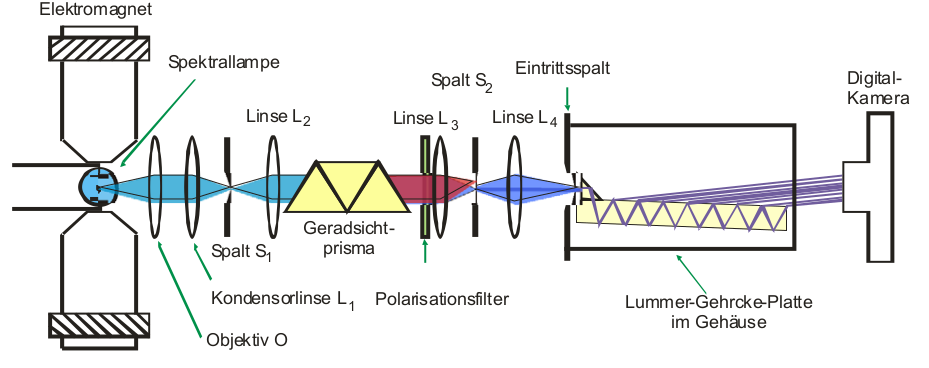
\includegraphics[width=0.98\columnwidth]{pictures/aufbau.png}
  \caption{Prinzipieller Aufbau des Versuchs.\cite{Anleitung}}
  \label{fig:aufbau}
\end{figure}
Das Objektiv $O$ und die Linse $L_1$ sorgen hierbei dafür, dass ein möglichst großer Teil des Lichts der Cd-Lampe auf den Spalt $S_1$ fokussiert wird.\\
Der Lichtstrahl wird durch die Linse $L_2$ kollimiert und kann anschließend im Geradsichtprisma spektral zerlegt, ohne dass sich die Richtung seiner optischen Achse ändert.
Mit dem folgenden Polarisationsfilter lässt sich die Polarisation des Lichtstrahls einstellen. \\
Anschließend fokussiert die Linse $L_3$ den Strahl auf den Spalt $S_2$. Dieser dient dazu, eine bestimmte Wellenlänge des Spektrums auszuwählen, die untersucht werden soll.\\ Schließlich fokussiert die Linse $L_4$ den Lichtstrahl auf den Eintrittsspalt der Lummer-Gehrcke-Platte.\\
Der Lichtstrahl trifft danach auf das Eintrittsprisma der Lummer-Gehrcke-Platte. Diese ist so zu justieren, dass der Lichtstrahl möglichst unter einem Winkel nahe der Totalreflexion an den planparallelen Platten gebrochen wird. \\
Anschließend kann
das von der Lummer-Gehrcke-Platte erzeugte
Interferenzmuster mit einer dahinter angebrachten Kamera aufgenommen werden.
